\documentclass{article}

\usepackage[T2A]{fontenc}
\usepackage[utf8]{inputenc}
\usepackage[russian]{babel}
\parindent 0pt
\parskip 8pt
\usepackage{setspace}
\usepackage{amsmath}
\usepackage{amssymb}
\usepackage{amsfonts}
\usepackage[left=2.3cm, right=2.3cm, top=2.7cm, bottom=2.7cm, bindingoffset=0cm]{geometry}
\usepackage{latexsym}
\usepackage[unicode, pdftex]{hyperref}
\usepackage{xcolor}
\usepackage{graphicx}
\graphicspath{ {./images/} }

\doublespacing

\begin{document}

\newcommand{\PG}[0]{\Pi\Gamma}

\tableofcontents

\newpage

\part{Определения}

	\newpage
	
	\section{Первообразная, неопределенный интеграл}
	
		\subsection{Первообразная}
	
			$f: \langle a, b \rangle \rightarrow \mathbb{R}$
	
			$F: \langle a, b \rangle \rightarrow \mathbb{R}$ ~--- первообразная $f$ на $\langle a, b \rangle$, если для любого $x \in \langle a, b \rangle$, $F$ ~--- дифференцируема в точке $x$, и $F'(x) = f(x)$.
	
			\underline{Пример}
	
			$f(x) = \sin{x} \Leftrightarrow F(x) = -\cos{x} + C$
	
		\subsection{Неопределенный интеграл}
	
			Неопределенным интегралом функции $f$ на $\langle a, b \rangle$ называют множество всех её первообразных.
			
			Обозначение: $\int{f}$, $\int{f(x) dx} = \left\{ F + C, C \in \mathbb{R} \right\}$, где $F$ ~--- любая первообразная.
		
	\newpage
		
	\section{Теорема о существовании первообразной}
		
		Пусть $f$ непрерывна на $\langle a, b \rangle \Rightarrow$ существует такая функция $F$ на $\langle a, b \rangle$, что $F' = f$.
		
		\textbf{Доказательство}
			
		В кредит
			
	\newpage
		
	\section{Таблица первообразных}
		
		\begin{enumerate}
			
			\item $f(x) = k$, $F(x) = kx$
				
			\item $f(x) = x^n$, $F(x) = \frac{x^{n + 1}}{n + 1}$
				
			\item $f(x) = \frac{1}{x}$, $F(x) = \ln |x|$
				
			\item $f(x) = e^x$, $F(x) = e^x$
				
			\item $f(x) = a^x$, $F(x) = \frac{a^x}{\ln a}$
				
			\item $f(x) = \sin{x}$, $F(x) = -\cos{x}$
				
			\item $f(x) = \cos{x}$, $F(x) = \sin{x}$
				
			\item $f(x) = \frac{1}{\sin^2{x}}$, $F(x) = -\ctg{x}$
				
			\item $f(x) = \frac{1}{\cos^2{x}}$, $F(x) = \tg{x}$
				
			\item $f(x) = \frac{1}{\sqrt{1 - x^2}}$, $F(x) = \arcsin{x}$
				
			\item $f(x) = \frac{1}{1 + x^2}$, $F(x) = \arctg{x}$
			
			\item $f(x) = \frac{1}{\sqrt{x^2 + 1}} = \ln (x + \sqrt{x^2 + 1})$
			
				
		\end{enumerate}
			
	\newpage
		
	\section{Равномерная непрерывность}
		
		Функция $f : \langle a, b \rangle \rightarrow \mathbb{R}$ равномерно непрерывна на $\langle a, b \rangle$, если:
			
		$\forall \varepsilon > 0$ $\exists \delta > 0$, $\forall x_0, x$ : $|x - x_0| < \delta$, $|f(x) - f(x_0)| < \varepsilon$
			
	\newpage
		
	\section{Площадь, аддитивность площади, ослабленная аддитивность}
		
		\subsection{Первое определение площади}
			
			Пусть $E$ ~--- множество всех ограниченных подмножество в $\mathbb{R}^2$ (или множество всех фигур).
			
			Тогда площадь ~--- это функция $\sigma$ : $E \rightarrow [0, +\infty)$ со свойствами:
			
			\begin{enumerate}
			
				\item аддитивность
				
					Если $A = A_1 \sqcup A_2 \Rightarrow \sigma(A) = \sigma(A_1) + \sigma(A_2)$
				
				\item нормировка
				
					$\sigma(\langle a, b \rangle \times \langle c, d \rangle) = (d - c)(b - a)$ 
		
			\end{enumerate}
			
			\underline{Замечание}
			
				Площадь монотонна, то есть если:	
			
				$A \subset B \Rightarrow \sigma(A) \leq \sigma(B)$
			
				$\sigma($вертикального отрезка$) = 0$
				
		\subsection{Второе определение площади}
			
			$\sigma : E \rightarrow [0, +\infty)$
				
			\begin{itemize}
				
				\item монотонна
					
				\item нормировка
					
				\item ослабленная аддитивность:
					
					$E = E_1 \cup E_2$, $E_1 \cap E_2$ ~--- вертикальный отрезок, $E_1$ и $E_2$ ~--- по разные стороны этого отрезка.
					
					$\sigma(E) = \sigma(E_1) + \sigma(E_2)$
						
			\end{itemize}
	
	\newpage
	
	\section{Положительная и отрицательная срезки}
	
	    \subsection{Определение}
	    
	        Пусть $f : \langle a, b \rangle \rightarrow \mathbb{R}$
	    
	        $f_+ (x) = \max (f(x), 0)$ ~--- положительная срезка
	    
	        $f_- (x) = \max (-f(x), 0)$ ~--- отрицательная срезка
	    
	    \subsection{Некоторые свойства}
	    
	        \begin{itemize}
	    
	            \item $f = f_+ - f_-$
	        
	            \item $f_+ + f_- = |f|$
	        
	        \end{itemize}
	    
	    \subsection{Подграфик}
	    
            Пусть $E \subset \langle a, b \rangle$
        
            $f(E) \geq 0$
        
            Тогда $\PG(f, E)$ ~--- подграфик $f$ на $E$, если:
        
	        $\PG (f, E) = \left\{ (x, y) \in \mathbb{R}^2, x \in F, 0 \leq y \leq f(x) \right\}$
	    
	\newpage

	\section{Определённый интеграл}

        \subsection{Определение}
        
            Определённым интегралом функции $f$ по промежутку $[a, b]$ называется: $f: \langle c, d \rangle \rightarrow \mathbb{R}$, $[a, b] \subset \langle c, d \rangle$
        
            $\int^b_a f(x)dx = \sigma (\PG (f_+, [a, b])) - \sigma (\PG (f_-, [a, b]))$
		
		\subsection{Замечание}
		
		    \begin{enumerate}
		    
		        \item $f \geq 0 \Rightarrow \int^b_a f \geq 0$
		        
		    	\item $f \equiv c \Rightarrow \int^b_a f = c(b - a)$
		        
		        	$c = 0$ ~--- очевидно
		            
		            $c > 0$ $\int^b_a = \sigma(\PG(c, [a, b])) = c(b - a)$
		            
		            $c < 0$ $\int^b_a = -\sigma(\PG(f_-, [a, b])) = -(-c)(b - a) = c(b - a)$
		            
		       \item $\int^b_a -f = - \int^b_a f$
		       
		       		$(-f)_+ = f_-$
		       		
		       		$(-f)_- = f_+$
		       		
		       \item Можно считать, что разрешён случай, когда $a = b$
		       
		       		$\int^b_a f = 0$
		       				
		    \end{enumerate}

	\newpage

	\section{Кусочно-непрерывная функция}
	
		Пусть $f$ всюду непрерывна на $[a, b]$ кроме конечного числа точек, все точки разрыва I рода. Тогда $f$ называют кусочно-непрерывной функцией.
		
	\newpage
	
	\section{Почти первообразная}
	
		Пусть $f$ ~--- кусочно-непрерывная функция на $[a, b]$. Тогда $F : [a, b] \rightarrow \mathbb{R}$ ~--- почти первообразная, если
		
		$\exists F'(x)$, $F'(x) = f(x)$ для всех $x$ кроме конечного числа точек и $F(x)$ ~--- непрерывна на $[a, b]$
		
\newpage
	
\part{Теоремы}

	\newpage
	
	\section{Теорема Кантора о равномерной непрерывности}
	
		Пусть $f: X \rightarrow Y$ ~--- метрические пространства, $f$ непрерывна на $X$, $X$ ~--- компактно. Тогда $f$ ~--- равномерное непрерывно на $X$.
		
		\textbf{Доказательство (от противного)}
		
			Воспользуемся тем свойством, что если $X$ ~--- компактно, то $X$ и секвенциально компактно.
			
			Предположим противное:
			
			$\exists \varepsilon > 0$ \textcolor{gray}{$\delta = \frac{1}{n}$} $\exists x_n,  \widetilde{x_n}$: $\rho(x_n, \widetilde{x_n}) < \frac{1}{n}$ $\rho(f(x_n), f(\widetilde{x_n})) \geq \varepsilon$
			
			Тогда выберем сходящуюся подпоследовательность из $x_n$ $x_{n_k} \rightarrow a \in X$, $\widetilde{x_{n_k}} \rightarrow a \in X$.
			
			Тогда $f(x_{n_k}) \rightarrow f(a)$ и $f(\widetilde{x_{n_k}}) \rightarrow f(a)$, то
			
			$\rho(f(x_{n_k}), f(\widetilde{x_{n_k}})) \rightarrow 0$ (по неравенству треугольника)
			
			Что и противоречит изначальному условию.

	\newpage
	
	\section{Теорема Брауэра о неподвижной точке}
	
		Пусть $f: B(0, 1) \subset \mathbb{R}^m \rightarrow B(0, 1)$ ~--- непрерывное, тогда
		
		$\exists x_0 : f(x_0) = x_0$
		
		\textbf{Доказательство}
		
		\subsection{Игра ''Гекс''}
		
			Пусть есть поле $n \times m$, состоящее из правильных шестиугольников (гексов). Также два игрока на каждом своём ходу красят гексы в белый или чёрный цвет. Тогда для любой раскраски найдётся либо чёрная тропинка, соединяющая верхнюю и нижнюю часть поля, либо белая тропинка, соединяющая левую и правую часть поля.
			
			Доказывается от противного
		
			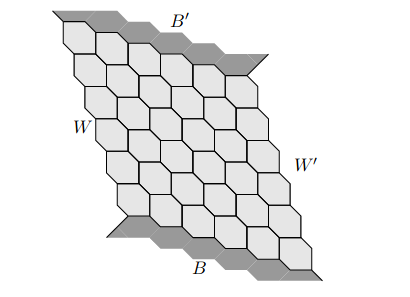
\includegraphics[scale=0.5]{HEX.png}
				
		\subsection{Сама теорема}
		
			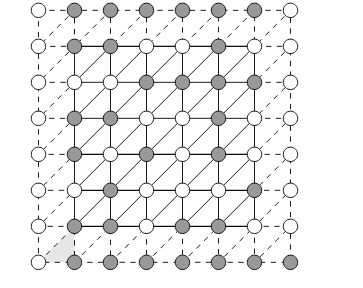
\includegraphics[scale=0.45]{NEWHEX.png}
		
			Теперь заменим гексы на обычную координатную плоскость, причём игра, по сути, останется такой же. Теперь перейдём к самой теореме.
			
			Шар с лёгкостью заменяется на обычный квадрат $[0, 1] \times [0, 1]$
			
			Пусть $f : [0, 1]^2 \rightarrow [0, 1]^2$ ~--- непрерывна. Тогда
			
			$\exists a \in [0, 1]^2$, $f(a) = a$
			
			$a \in [0, 1]^2$
			
			$a = (a_1, a_2)$
			
			$f(x) \in \mathbb{R}^2$
			
			$f(x) = (f(x)_1, f(x)_2)$
			
			\textbf{Доказательство}
			
				Пусть $\rho$ ~--- функция, заданная на $[0, 1]^2 \times [0, 1]^2$
				
				$\rho(x, y) = \max (|x_1 - y_1|, |x_2 - y_2|)$ ~--- непрерывна на $[0, 1]^2$
				
				$x_n \rightarrow a$
				
				$y_n \rightarrow b$
				
				$\rho(x_n, y_n) \rightarrow \rho(a, b)$
				
				Очевидно, что для любых $x, y: x \neq y \Rightarrow \rho(x, y) > 0$
				
				\underline{Теперь к самой теореме}
				
				Пусть для любого $x \in [0, 1]^2$ $f(x) \neq x$. Тогда $\rho(x, f(x)) > 0$, но $\rho$ непрерывно по $x$ и $[0, 1]^2$ ~--- компакт, значит по теореме Вейерштрасса существует такое $\varepsilon > 0$, что
				
				$\min\limits_{x \in [0, 1]^2} \rho(x, f(x)) = \varepsilon > 0$
				
				По теореме Кантора для этого $\varepsilon$ найдётся такая $\delta$ (будем считать, что $\sqrt{2} \delta < \varepsilon$), что
				
				$\forall x, \widehat{x} \in [0, 1]^2 : \| x - \widehat{x} \| < \delta \cdot \sqrt{2} \Rightarrow \| f(x) - f(\widehat{x}) \| < \varepsilon$
				
				Берём $\frac{1}{n} < \varepsilon$
				
				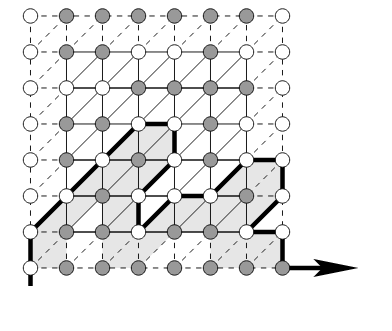
\includegraphics[scale=0.45]{HEXTHEOREM.png}
				
				\underline{Доска}
				
				Узел $(l, k) \rightarrow (\frac{l}{n}, \frac{k}{n}) \in [0, 1]^2$
				
				$0 \leq l, k \leq n$
				
				Красим узлы
				
				$v$ ~--- логический узел, $v = (v_1, v_2)$
				
				$c(v) = \min \left\{ i : \left\| f(\frac{v}{n})_i - \frac{v_i}{n} \right\| \geq \varepsilon \right\}$
			
				По лемме об игре в гексы есть одноцветная тропинка.
				
				Путь $v^0$ ~--- начальная точка тропинки, $v^N$ ~--- конечная.
				
				$v^0_1 = 0$
				
				$f(\frac{v^0}{n}) \in [0, 1]^2$, т.е. $f(\frac{v^0}{n})_1 \geq 0$
				
				$\varepsilon \leq f(\frac{v^0}{n})_1$
				
				Аналогично для $v^N_1 = 1$
				
				$f(\frac{v^N}{n})_1 \leq 1$
				
				$f(\frac{v^N}{n})_1 - \frac{v^N_1}{n} \leq -\varepsilon$
				
				$f(\frac{v^0}{n})_1 - \frac{v^0_1}{n} \geq \varepsilon$
	
				Поскольку для любых $x$ верно, что $|f(x)_1 - x_1| \geq \varepsilon$, то из этого следует, что какой-то прыжок был длиной не меньше $2 \varepsilon$, но такое невозможно, поскольку по условию если $\| x - \widehat{x} \| < \frac{1}{n} \Rightarrow \| f(x) - f(\widehat{x}) \| < \varepsilon$
				
				
	\newpage

	\section{Теорема о свойствах неопределенного интеграла}
	
		Пусть $f$, $g$ имеют первообразную на $\langle a, b \rangle$. Тогда:
		
		\begin{enumerate}
		
			\item $\int f + \int g  = \int (f + g)$
			
				$\forall \alpha \in \mathbb{R}$ $\int(\alpha f) = \alpha \int{f}$
				
			\item $\forall \varphi: \langle c, d \rangle \rightarrow \langle a, b \rangle$, $\varphi$ дифференцируема
			
				$\int f(\varphi(t))\varphi'(t)dt = F(\varphi(t)) + C$, где $F$ ~--- первообразная $f$
				
			\item $\forall \alpha, \beta \in \mathbb{R}$, $\alpha \neq 0 : \int f(\alpha x + \beta)dx = \frac{1}{\alpha} F(\alpha x + \beta) + C$
			
			\item $f$, $g$ ~--- дифференцируемы на $\langle a, b \rangle$
			
				$f' \cdot g$ имеет первообразную на $\langle a, b \rangle$
				
				Тогда $f \cdot g'$ тоже имеет первообразную и 
				
				$\int f'g = fg - \int fg'$
				
		\end{enumerate}
			
		\textbf{Доказательство}
		
		\begin{enumerate}
		
			\item $(F + G)' = f + g$
			
				$(\alpha F)' = \alpha f$
				
			\item $(F(\varphi(t)))' = f(\varphi(t))\varphi'(t)$
			
			\item $(\frac{1}{\alpha} F (\alpha x + \beta))' = f(\alpha x + \beta)$
			
			\item $(fg)' = f'g + fg'$, т.е. $fg = \int f'g + \int fg'$
			
		\end{enumerate}
		
	\newpage
	
	\section{Интегрирование неравенств. Теорема о среднем}
	
		\subsection{Интегрирование неравенств}
		
			Пусть $f$, $g \in C[a, b]$, $f \leq g \Rightarrow \int\limits^b_a f \leq \int\limits^b_a g$
			
			Если $0 \leq f \leq g$
			
			$\int\limits^b_a f = \sigma (\PG (f, [a, b])) \leq \sigma (\PG (g, [a, b])) = \int\limits^b_a g$
			
			В общем случае
			
			$\PG(f_+, [a, b]) \subset \PG(g_+, [a, b])$
			
			$\PG(f_-, [a, b]) \supset \PG(g_-, [a, b])$
			
			$\sigma (\PG(f_+, [a, b])) - \sigma (\PG(f_-, [a, b])) \leq \sigma (\PG(g_+, [a, b])) - \sigma (\PG(g_-, [a, b]))$
			
			$\int\limits^b_a f \leq \int^b_a g$
			
		\subsection{Теорема о среднем значении}
		
			Пусть $f$ непрерывна на $[a, b] \Rightarrow \exists c \in [a, b]: \int\limits^b_a f = f(c)(b-a)$
		
		\subsection{Доказательство 1}
		
			Просто берём прямую и двигаем её сверху вниз, тем самым по теореме о бутерброде мы найдём такое значение $c$, что $\int\limits^b_a f = f(c)(b - a)$
			
		\subsection{Нормальное доказательство}
		
			Если $a = b$ ~--- очевидно.
			
			Пусть $a < b$
			
			$\min f \leq \frac{1}{b - a} \int\limits^b_a f \leq \max f$
			
			по теореме о промежуточном значении
			
			$\exists c : \frac{1}{b - a} \int\limits^b_a f = f(c)$
			
	\newpage
	
	\section{Теорема Барроу}
	
		\subsection{Определение}
		
			$f \in C[a, b]$, $\varphi : [a, b] \rightarrow \mathbb{R}$
		
			$\varphi (x) = \int\limits^x_a f(t)dt$
		
			Интеграл с верхним переменным пределом
		
		\subsection{Теорема (Барроу)}
		
			В условиях определения оказывается, что $\varphi$ ~--- диффиринцируема на $[a, b]$ и $\varphi'(x) = f(x) \ \forall x \in [a, b]$
		
		\subsection{Доказательство}
		
			Фиксируем $x$ и при $y > x$
		
			$\lim\limits_{y \rightarrow x + 0} \frac{\varphi(y) - \varphi(x)}{y - x} = \lim\limits_{y \rightarrow x + 0} \frac{1}{y - x} ( \int\limits^y_a f - \int\limits^x_a f) = \lim\limits_{y \rightarrow x + 0} \frac{1}{y - x} \int\limits^y_x f = \lim\limits_{y \rightarrow x + 0} f(c) = f(x)$
		
			$\exists c \in [x, y]$
		
			Аналогично доказываем, что $\lim\limits_{y \rightarrow x - 0} = \ldots = f(c)$
		
		\subsection{Замечания}
		
			\begin{itemize}
			
				\item Интеграл с нижним переменным пределом
				
					$\psi(x) = \int\limits^b_x f$. Тогда $\psi'(x) = -f$
					
				\item Эта теорема также доказывает теорему о существовании производной
				
			\end{itemize}
			
	\newpage
	
	\section{Формула Ньютона-Лейбница, в том числе, для кусочно-непрерывных функций}
	
		\subsection{Формулировка теоремы}
		
			Пусть $f$ непрерывна на $[a, b]$, $F$ ~--- первообразная $f$. 
		
			Тогда $\int\limits^b_a f = F(b) - F(a)$
		
		\subsection{Доказательство}
		
			$\varphi$ ~--- из теоремы Барроу ~--- тоже первообразная, значит
			
			$\exists c$ $F = \varphi + c$
			
			$\int\limits^b_a f = \varphi(b) = \varphi(b) - \varphi(a) = (\varphi + c) \bigg|_{x = b} - (\varphi + c) \bigg|_{x = a} = F(b) - F(a)$
			
			$\int\limits^b_a f = F(b) - F(a)$
			
			При $a > b$ $\int\limits^b_a f \stackrel{\mathrm{def}}{=} - \int\limits^a_b f$
			
	\newpage
	
	\section{Свойства определенного интеграла: линейность, интегрирование по частям, замена переменных}
	
		\subsection{Линейность определенного интеграла}
		
			$f, g \in C[a, b]$, $\alpha$, $\beta \in \mathbb{R}$
			
			$\int\limits^b_a \alpha f + \beta g = \alpha \int\limits^b_a f + \beta \int\limits^b_a g$
			
			Следует из формулы Ньютона-Лейбница
			
			$\int\limits^b_a f = F(b) - F(a) = F(x) \bigg|^b_a$
			
			$F$, $G$ $\alpha F + \beta G$ ~--- первообразная $\alpha f + \beta g$
			
			$\alpha F(x) + \beta G(x) \bigg|^b_a = \alpha F(b) + \beta G(b) - \alpha F(a) - \beta G(a) = \alpha (F(b) - F(a)) + \beta (G(b) - G(a)) = \alpha \int\limits^b_a f + \beta \int\limits^b_a g$
			
		\subsection{Интегрирование по частям}
		
			$f, y \in C^{}[a, b]$. Тогда
			
			$\int\limits^b_a f g' = fg \bigg|^b_a - \int\limits^b_a f'g$
			
			Следует из свойств для неопределенного интеграла
			
			$\int\limits^b_a f g' = (\int f g') \bigg|^b_a = (fg - \int f' g) \bigg|^b_a = fg \bigg|^b_a - \int\limits^b_a f'g$
		
		\subsection{Замена переменных}

			Пусть $f \in C(\langle a, b \rangle)$

			$\varphi : \langle \alpha, \beta \rangle \rightarrow \langle a, b \rangle$

			$\varphi \in C^1 (\langle a, b \rangle)$

			$[p, q] \in \langle \alpha, \beta \rangle$

			Тогда $\int\limits^q_p f(\varphi(t))\varphi'(t) \ dt = \int\limits^{\varphi(q)}_{\varphi(q)} f(x) \ dx$

			\underline{Доказательство}

			Пусть $F$ ~--- первообразная $f$
	
			$F(\varphi(t))$ ~--- первообразная $f(\varphi(t))\varphi'(t)$ на $[p, q]$

			Тогда обе части: $F(\varphi(q)) - F(\varphi(p))$

			\underline{Замечание}

			\begin{enumerate}

				\item Возможен случай $\varphi([p, q]) \supset [\varphi(p), \varphi(q)]$

				\item В другую сторону

					$\int\limits^v_u f(x) \ dx = \int\limits^q_p f(\varphi(t))\varphi'(t) \ dt$

					Тогда подбираем такие $p$ и $q$, что когда $t$ ходит от $p$ до $q$ $\varphi(t)$ ходит от $v$ до $u$

			\end{enumerate}
	\newpage
	
	\section{Интегральное неравенство Чебышева. Неравенство для сумм}
	
		\subsection{Формулировка}
		
			$I_f = \frac{1}{b - a} \int\limits^b_a f$
		
			$f, g \in C[a, b]$ ~--- монотонно возрастают
			
			Тогда $I_f \cdot I_y \leq I_{fg}$
		
			$\int\limits^b_a f \cdot \int\limits^b_a g \leq (b - a) \int\limits^b_a fg$ ~--- неравенство Чебышева
		
		\subsection{Доказательство}
		
			$\forall x, y \in [a, b]$ $(f(x) - f(y))(g(x)-g(y)) \geq 0$
			
			Проинтегрируем по переменной $x$ по отрезку $[a, b]$
			
			$f(x)g(x) - f(y)g(x) - f(x)g(y) + f(y)g(y) \geq 0$
			
			$I_{fg} - f(y)I_g - I_f g(y) + f(y)g(y) \geq 0$
			
			Интегрируем по $y$ на $[a, b] : \frac{1}{b - a} \int\limits^b_a$
			
			$I_{fg} - I_f \cdot I_g - I_f \cdot I_g + I_{fg} \geq 0$
			
			$I_{fg} \geq I_f \cdot I_g$
	
	\newpage
	
	\section{Иррациональность числа $\pi$}
	
		\subsection{Вспомогательный интеграл}
		
			Пусть $H_n = \frac{1}{n!} \int\limits^{\frac{\pi}{2}}_{-\frac{\pi}{2}} (\frac{\pi^2}{4}-t^2)^n \ \cos t \ dt$
			
			$H_n = \begin{bmatrix} f = (\frac{\pi^2}{4} - t^2)^n & g = \sin t \\ f' = -2nt (\frac{\pi^2}{4} - t^2)^{n - 1} & g' = -\cos t \end{bmatrix}$
			
			$H_n = \frac{1}{n!} (\frac{\pi^2}{4} - t^2)^n \sin t \bigg|^{\frac{\pi}{2}}_{-\frac{\pi}{2}} + \frac{1}{n!} 2n \int\limits^{\frac{\pi}{2}}_{-\frac{\pi}{2}} t (\frac{\pi^2}{4}-t^2)^{n - 1} \sin t \ dt$
			
			$H_n = \frac{1}{n!} 2n \int\limits^{\frac{\pi}{2}}_{-\frac{\pi}{2}} t (\frac{\pi^2}{4}-t^2)^{n - 1} \sin t \ dt$
			
			$H_n = \begin{bmatrix} f = t (\frac{\pi^2}{4} - t^2)^{n - 1} & g = -\cos t \\ f' = (\frac{\pi^2}{4} - t^2)^{n - 1} - 2(n - 1)t^2(\frac{\pi^2}{4} - t^2)^{n - 2} & g' = \sin t \end{bmatrix}$
			
			$f' = (\frac{\pi^2}{4} - t^2)^{n - 1} + 2(n - 1)(\frac{\pi^2}{4} - t^2)^{n - 1} - \frac{\pi^2}{2} (n - 1) (\frac{\pi^2}{4} - t^2)^{n - 2}$
			
			$f' = (2n - 1)(\frac{\pi^2}{4} - t^2)^{n - 1} - \frac{\pi^2}{2}(n - 1)(\frac{\pi^2}{4}-t^2)^{n - 2}$
			
			$\frac{2}{(n - 1)!} t (\frac{\pi^2}{4} - t^2)^{n - 1} (-\cos t) \bigg|^{\frac{\pi}{2}}_{-\frac{\pi}{2}} - \frac{2}{(n - 1)!} \int\limits^{\frac{\pi}{2}}_{-\frac{\pi}{2}} ( (2n - 1)(\frac{\pi^2}{4} - t^2)^{n - 1} - \frac{\pi^2}{2} (n - 2) (\frac{\pi^2}{4} - t^2)^{n - 2}) \cos t \ dt$
			
			Пусть $n \geq 2$, тогда
			
			$H_n = (4n - 2) H_{n - 1} - \pi^2 H_{n - 2} = \ldots + H_2 + \ldots + H_0$
			
			$H_0 = 2$
			
			$H_1 = 2 \int\limits^{\frac{\pi}{2}}_{-\frac{\pi}{2}} \frac{t}{f} \frac{g'}{\sin t} = 2t (- \cos t)\bigg|^{\frac{\pi}{2}}_{-\frac{\pi}{2}} + 2 \int\limits^{\frac{\pi}{2}}_{-\frac{\pi}{2}} \cos t \ dt = 4$
			
		\subsection{Теорема}
		
			Число $\pi^2$ ~--- иррациональное (и тогда $\pi$ тоже)
			
		\subsection{Доказательство}
		
			Пусть $\frac{1}{n!} \int\limits^{\frac{\pi}{2}}_{-\frac{\pi}{2}} (\frac{\pi^2}{4} - t^2)^n \cos t = P_n (\pi^2)$, где $P_n$ ~--- многочлен с целыми коэффициентами.
			
			$\deg P \leq n$
			
			Этого не может быть
			
			\underline{От противного}
			
			Пусть $\pi^2 = \frac{m}{k} \in \mathbb{Q}$. Тогда $k^n P_n(\frac{m}{k})$ ~--- целое число
			
			Значит $k^n \cdot P_n (\frac{m}{k}) \geq 1$, т.е.
			
			$\frac{k^n}{n!} \int\limits^{\frac{\pi}{2}}_{-\frac{\pi}{2}} (\frac{\pi^2}{4} - t^2)^n \cos t \ dt \geq 1$
			
			$\frac{k^n}{n!} \int\limits^{\frac{\pi}{2}}_{-\frac{\pi}{2}} (\frac{\pi^2}{4} - t^2)^n \cos t \ dt \leq \frac{k^n}{n!} (\frac{\pi^2}{4})^n \cdot \pi \xrightarrow[n \rightarrow +\infty]{} 0$
			
	\newpage
	
	\newpage

	\section{Формула Тейлора с остатком в интегральной форме}


		\subsection{Формулировка}

			Пусть $\langle a, b \rangle \in \overline{\mathbb{R}}$, $f \in c^{n + 1} (\langle a, b \rangle)$

			$x$, $x_0 \in \langle a, b \rangle$. Тогда

			$f(x) = \sum\limits^n_{k = 0} \frac{f^{(k)} (x_0)}{k!} (x - x_0)^k + \frac{1}{n!} \int\limits^x_{x_0} (x - t)^n f^{(n + 1)}(t) \ dt$

		\subsection{Доказательство}

			\underline{По индукции}

			\begin{itemize}

				\item $n = 0 : f(x) = f(x_0) = \int\limits^x_{x_0} f'(t) \ dt$

					По формуле Ньютона-Лейбница

				\item Переход от $n$ к $n + 1$

					$f(x) + T_n + \frac{1}{n!} \int\limits^x_{x_0} (x - t)^n f^{(n + 1)} (t) \ dt = \begin{bmatrix} u' (x - t)^n & u = -\frac{(x - t)^{n + 1}}{n + 1} \\ v = f^{n - 1} & v' = f^{(n + 2)} \end{bmatrix}$
						
					$T_n + \frac{1}{n!} \left( -\frac{(x - t)^{n + 1}}{(n + 1)} \cdot f^{(n + 1)} (t) \bigg|^{t = x}_{t = x_0} + \int\limits^x_{x_0} \frac{(x - t)^{n + 1}}{n + 1} \cdot f^{(n + 2)} (t) \ dt \right)$ 
					
					$T_n + \frac{f^{(n + 1)} (x_0)}{(n + 1)!} (x - x_0)^{n + 1} + \frac{1}{(n + 1)!} \int\limits^x_{x_0} (x - t)^{n + 1} f^{(n + 2)} (t) \ dt$

			\end{itemize}

		\subsection{Послесловие}

			$f(x) = \sum\limits^n_{k = 0} \frac{f^{(k)}(x_0)}{k!} (x - x_0)^k + R_n$

			$f(t) = \sum\limits^n_{k = 0} \frac{f^{(k)}(x_0)}{k!} (t - x_0)^k + R_n$

			$F$ ~--- первообразная $f$  $\int\limits^x_{x_0} f(t) \ dt = F(x) - F(x_0)$

			$F(x) - F(x_0) = \sum\limits^n_{k = 0} \int\limits^x_{x_0} \frac{f^{(k)} (x_0)}{k!} (t - x_0)^k \ dt + \int\limits^x_{x_0} R_n = \frac{(t - x_0)^{k + 1}}{k + 1} \bigg|^{t = x}_{t = x_0}$

			$\sum\limits^n_{k = 0} \frac{F^{(k + 1)} (x_0)}{(k + 1)!} (x - x_0)^{k + 1} + \int\limits^x_{x = 0} R_n$

			Мы имеем право формально интегрировать формулу Тейлора

	\newpage

	\section{Лемма об ускоренной сходимости}
	
		\subsection{Формулировка}
		
			Пусть $f$, $g : D \rightarrow \mathbb{R}$, $a$ ~--- предельная точка $D \subset \mathbb{R}$, $a \in \overline{\mathbb{R}}$
		
			Пусть также существует $U(a) : f(a) \neq 0$ и $g(a) \neq 0$ в $\dot{U}(a)$
		
			Пусть $\lim\limits_{x \rightarrow a} f(x) = 0$ и $\lim\limits_{y \rightarrow a} g(x) = 0$ (Также возможен вариант, что $\lim\limits_{x \rightarrow a} f(x) = + \infty$ и $\lim\limits_{y \rightarrow a} g(x) = +\infty$)
			
			Тогда для любой последовательности $x_k \rightarrow a$, $x_k \in D$, $x_k \neq a$ найдётся такая последовательность $y_k \rightarrow a$ ($y_k \in D$, $y_k \neq a$), что 
			
			$\lim\limits_{k \rightarrow +\infty} \frac{f(y_k)}{g(x_k)} = 0$ и $\lim\limits_{k \rightarrow +\infty} \frac{f(y_k)}{f(x_k)} = 0$
			
		\subsection{Доказательство}
		
			\begin{enumerate}
			
				\item Пусть $f$, $g \rightarrow 0$, тогда можно добиться того, что $\left| \frac{f(y_k)}{f(x_k)} \right| < \frac{1}{k}$ и $\left| \frac{f(y_k)}{g(x_k)} \right| < \frac{1}{k}$
			
					Тогда найдётся такое $K$, что $\left| \frac{f(x_k)}{f(x_{2019})} \right| < \frac{1}{2019}$ для любых $k > K \Rightarrow y_{2019} = x_k$
			
					Продолжаем так до бесконечности
			
					$\left| \frac{f(x_i)}{f(x_k)} \right| < \frac{1}{k}$
			
					$\exists i > k$ $\left| \frac{f(x_i)}{f(x_k)} \right| < \frac{1}{k} \Rightarrow y_k := x_i$

					Теперь пусть $\left| \frac{f(x_i)}{g(x_k)} \right| < \frac{1}{k}$ при $x \rightarrow +\infty$ и $\left| \frac{f(x_i)}{g(x_k)} \right| < \frac{1}{k}$ также при $i \rightarrow +\infty$
			
					Тогда для каждого $k$ найдётся такое $K$, что для всех $i > K$ выполняется сразу оба условия, значит присвоим $y_k := x_i$, где $i$ ~--- какое-то число большее $K$.
		
				\item Пусть $f$, $g \rightarrow +\infty$. Считаем, что $f > 0$ и $g > 0$. Пусть $f(x_k)$ и $g(x_k)$ ~--- возрастающие последовательности (остальные случаи рассматриваются аналогично). Тогда
				
					$i = \min n: \begin{cases} f(x_n) \geq \sqrt{g(x_k)} \\ f(x_n) \geq \sqrt{f(x_k)} \end{cases}$
					
					Возьмём $y_k := x_{i - 1}$
					
					Тогда $\frac{f(y_k)}{f(x_k)} < \frac{\sqrt{f(x_k)}}{f(x_k)} = \frac{1}{\sqrt{f(x_k)}} \rightarrow 0$
					
						$\frac{f(y_k)}{g(x_k)} < \frac{\sqrt{g(x_k)}}{g(x_k)}= \frac{1}{\sqrt{g(x_k)}} \rightarrow 0$
					
			\end{enumerate}	
			
	\newpage
	
	\section{Правило Лопиталя (с леммой)}
	
		\subsection{Формулировка}
			
			Пусть $f$, $g$ ~--- дифференцируемы на $(a, b \rangle$, $g' \neq 0$ на $(a, b \rangle$ и существует $\lim\limits_{x \rightarrow a} \frac{f'(x)}{g'(x)} = A \in \overline{\mathbb{R}}$
			
			Тогда $\lim\limits{x \rightarrow a} \frac{f(x)}{g(x)} = A$
			
		\subsection{Пример из жизни}
		
			Пусть $f$, $g : [0, +\infty) \rightarrow \mathbb{R}$
			
			Пусть $f$ ~--- сколько прошёл студент, 	
			
				$g$ ~--- сколько прошёл Кохась.
				
			Тогда $f$, $g \rightarrow +\infty$, но если сравним скорости $f'$ и $g'$, то легко узнать, на сколько больше прошёл Кохась, чем студент.
			
		\subsection{Доказательство}
		
			$g' \neq 0 \Rightarrow g'$ сохраняет знак (по теореме Дарбу), значит $g$ ~--- строго монотонна
			
			\begin{enumerate}
			
				\item $g \rightarrow +\infty \Rightarrow g > 0$ в окрестности точки $a$
				
				\item $g \rightarrow 0$,
					
					$g \uparrow \ \Rightarrow g > 0$ в окрестности точки $a$
			
					$g \downarrow \ \Rightarrow g < 0$ в окрестности точки $a$
					
			\end{enumerate}
			
		\subsection{Собственное доказательство}
		
			Берём последовательность $y_k \rightarrow a$ из леммы.
			
			По теореме Коши $\exists \xi_k \in [x_k, y_k]$ (не факт, что $x_k \leq y_k$)
			
			$\frac{f(x_k) - f(y_k)}{g(x_k) - g(y_k)} = \frac{f'(\xi_k)}{g'(\xi_k)}$
			
			$\frac{f(x_k)}{g(x_k)} = \frac{f(y_k)}{g(x_k)} + \frac{f'(\xi_k)}{g'(\xi_k)} \left( 1 - \frac{g(y_k)}{g(x_k)} \right)$
			
			$\frac{f(x_k)}{g(x_k)} \rightarrow \frac{f'(\xi_k)}{g'(\xi_k)}$
			
	\newpage
	
	\section{Теорема Штольца}
	
		\subsection{Формулировка}
		
			Пусть $x_n$, $y_n \rightarrow 0$
			
			$\lim\limits_{n \rightarrow +\infty} \frac{x_n}{y_n} = \left[ \frac{0}{0} \right]$
			
			Тогда если существует $\lim\limits_{n \rightarrow +\infty} \frac{x_n - x_{n - 1}}{y_n - y{n - 1}} = a \in [0, +\infty]$
			
			Также $y_n$ ~--- строго монотонна (если $a = 0$, то $x_n$ ~--- тоже строго монотонна)
			
			Тогда $\exists \lim\limits_{n \rightarrow +\infty} \frac{x_n}{y_n} = a$
			
		\subsection{Доказательство}
		
			\begin{enumerate}
			
				\item Пусть $a > 0$, $a$ ~-- конечное, тогда можно считать, что $y_n \geq y_{n - 1}$ из монотонности и $x_n \geq x_{n - 1}$ при больших $n$.
			
					Заметим обидный факт, что $\frac{a}{b} \cdot \frac{c}{d} = \frac{ac}{bd}$ и $\frac{a}{b} : \frac{c}{d} = \frac{a : c}{b : d}$, но $\frac{a}{b} + \frac{c}{d} \neq \frac{a + c}{b + d}$. Кохасю обидно, поэтому будем считать, что $\frac{a}{b} + \frac{c}{d} = \frac{a + c}{b + d}$. Если вы с этим не согласны, то окей, но заметим, что справедливо:
			
					$0 < \alpha < \frac{a}{b} < \beta$
			
					$0 < \alpha < \frac{c}{d} < \beta$
			
					$\alpha < \frac{a + c}{b + d} < \beta$
			
					Вернёмся к самой теореме
			
					$\forall \varepsilon > 0$ $(\varepsilon < a)$ $\exists N_1$ $\forall n > N \geq N_1$
			
					$a - \varepsilon < \frac{x_{N + 1} - x_N}{y_{N + 1} - y_N} < a + \varepsilon$
			
					$a - \varepsilon < \frac{x_{N + 2} - x_{N + 1}}{y_{N + 2} - y_{N + 1}} < a + \varepsilon$
			
					$\vdots$
			
					$a - \varepsilon < \frac{x_n - x_{n - 1}}{y_n - y_{n - 1}} < a + \varepsilon$
			
					Складываем всё
			
					$a - \varepsilon < \frac{x_n - x_N}{y_n - y_N} < a + \varepsilon$
			
					Устремляем $n$ к $+\infty$
			
					$a - \varepsilon \leq \frac{x_N}{y_N} < a + \varepsilon$
			
				\item Если $a = +\infty$ ~--- аналогично
				
					$\forall E > 0$ $\exists N_1$, $\forall n > N \geq N_1$ $\frac{x_{N + 1} - x_{N}}{y_{N + 1} - y_N} > E$
					
					$E < \frac{x_n - X_N}{y_n - y_N}$
					
					$E \leq \frac{x_N}{y_N}$
					
				\item Если $a = 0$, то $\lim\limits_{n \rightarrow +\infty} \frac{y_n}{x_n} = +\infty$
				
				\item Если $a < 0$ ~--- меняем знаки
				
			\end{enumerate}						
		
	\newpage
	
	\section{Пример неаналитической функции}
	
		\subsection{Неалитическая функция}
		
			$f(x) = \begin{cases} e^{-\frac{1}{x^2}}, & x \neq 0 \\ 0, & x = 0 \end{cases}$
			
		\subsection{Утверждение}
		
			$f$ ~--- бесконечное дифференцируема на $\mathbb{R}$
			
			($\forall x \in \mathbb{R}$ $\forall k \in \mathbb{N}$ $\exists f^{(k)} (x)$)
			
		\subsection{Доказательство}
		
			Если $x \neq 0$ ~--- то очевидно
			
			Пусть $x = 0$, тогда для любого $k$ $\exists f^{(k)} (0) = 0$
			
			Из теоремы Лагранжа:
			
			Если $\exists \lim\limits_{x \rightarrow a + 0} f'(x) = \lim\limits_{x \rightarrow a - 0} f'(x) = L$, где $L \in \mathbb{R}$, то
			
			$f$ ~--- дифференцируема и $f'(a) = L$
			
			$f'(x) = \frac{2}{x^3} \cdot e^{-\frac{1}{x^2}}$, $x \neq 0$
			
			$\lim\limits_{x \rightarrow 0} \frac{\frac{1}{x^3}}{e^{\frac{1}{x^2}}} = \left[ \frac{\infty}{\infty} \right] = \lim\limits_{x \rightarrow 0} \frac{-\frac{3}{x^4}}{-\frac{2}{x^3} e^{\frac{1}{x^2}}} = \lim\limits_{x \rightarrow 0} \frac{3}{2} \cdot \frac{\frac{1}{x}}{e^{\frac{1}{x^2}}} = \lim\limits_{x \rightarrow 0} \frac{-\frac{1}{x^2}}{-\frac{2}{x^3} e^{\frac{1}{x^2}}} = \lim\limits_{x \rightarrow 0} \cdot x \cdot e^{-\frac{1}{x^2}} \rightarrow 0$
			
			$\lim\limits_{x \rightarrow 0} \frac{1}{x^k} \cdot e^{-\frac{1}{x^2}} = \left( \lim\limits_{x \rightarrow 0} \frac{\frac{1}{x^2}}{e^{\frac{1}{x^2} \cdot \frac{2}{k}}} \right)^{\frac{k}{2}} = \left( \lim\limits_{x \rightarrow 0} \frac{-\frac{1}{x^3}}{-\frac{4}{k} \cdot \frac{1}{x^3} \cdot e^{\frac{1}{x^3}}} \right)^\frac{k}{2} = 0$
			
			\underline{Итого}
			
			$f'(x) = \frac{2}{x^3} \cdot e^{-\frac{1}{x^2}}$, $x \neq 0$
			
			$f'(0) = 0$
			
			Аналогично
			
			$f'' = -\frac{6}{x^4} \cdot e^{-\frac{1}{x^2}} - \frac{4}{x^5} \cdot e^{-\frac{1}{x^2}}$, $x \neq 0$
			
			$\lim\limits_{x \rightarrow 0} f''(x) = 0 \Rightarrow f''(0) = 0$
			
			$x \neq 0$ $f^{(k)} (x) = P_k (\frac{1}{x}) \cdot e^{-\frac{1}{x^2}}$
			
			$\lim\limits_{x \rightarrow 0} f^{(k)}(x) = 0 \Rightarrow f^{(k)}(0) = 0$
			
			
\end{document}
